\documentclass{standalone}
\usepackage{tikz,pgfplots,calc}
\usetikzlibrary{positioning,calc}
\usetikzlibrary{arrows}
\usepackage{tkz-euclide}
\usetkzobj{all}
\renewcommand{\familydefault}{\sfdefault}

\begin{document}

\begin{tikzpicture}
% \node [label=below:a)] (n1) at (0, 0) {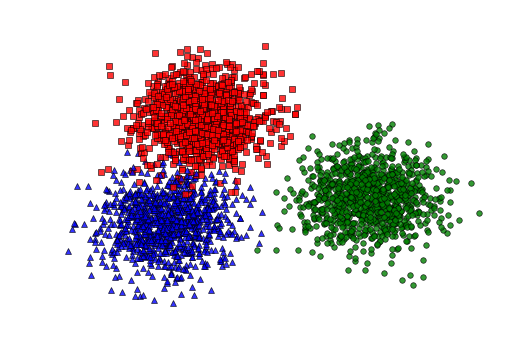
\includegraphics[width=4cm]{dist1.png}};
% \node (n2) [right=0cm of n1, label=below:b)] {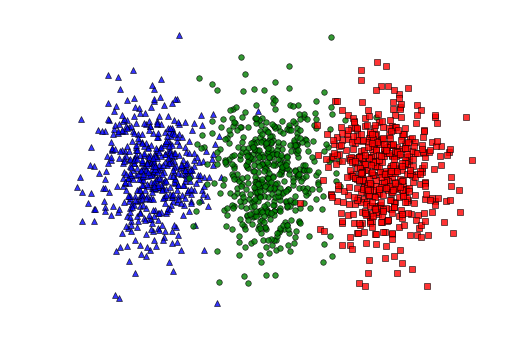
\includegraphics[width=4cm]{dist2.png}};
% \node (n3) [right=0cm of n2, label=below:c)] {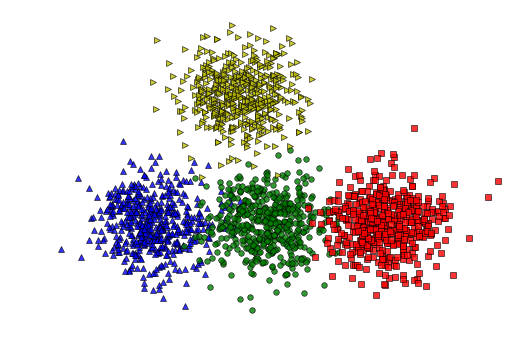
\includegraphics[width=4cm]{dist3.png}};

\def\d{6}
\node [label=below:a)] (n1) at (0, 0) {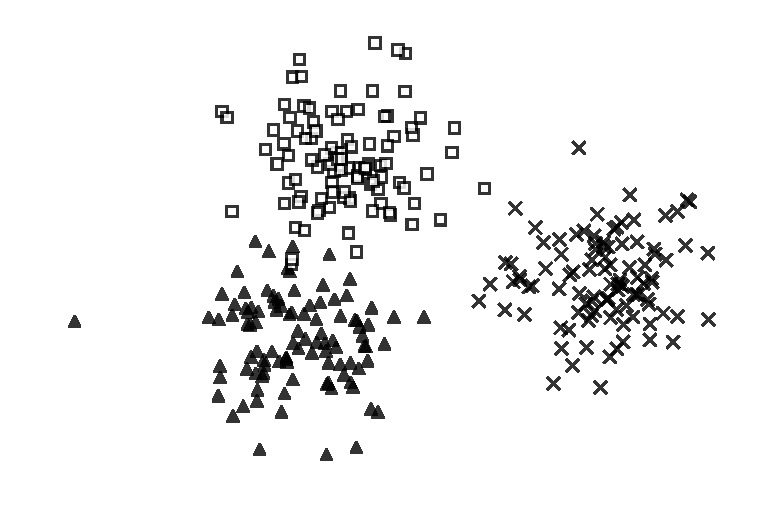
\includegraphics[width=\d cm]{dist1.pdf}};
\node (n2) [right=-1cm of n1, label=below:b)] {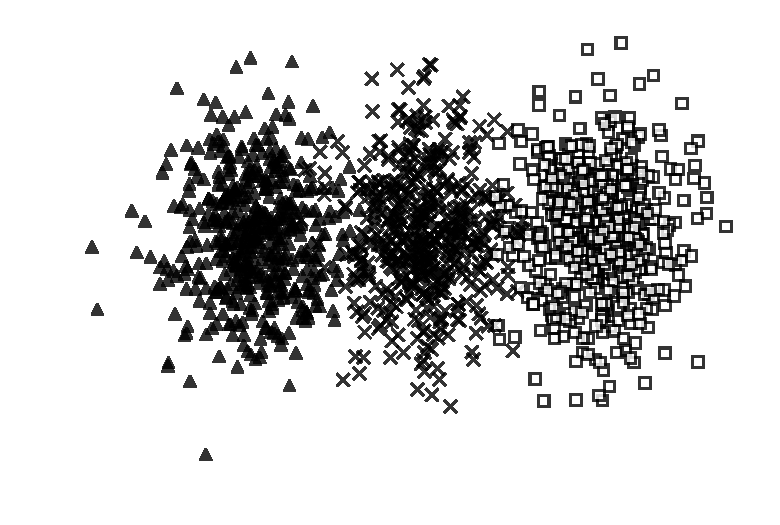
\includegraphics[width=\d cm]{dist2.pdf}};
\node (n3) [right=-1cm of n2, label=below:c)] {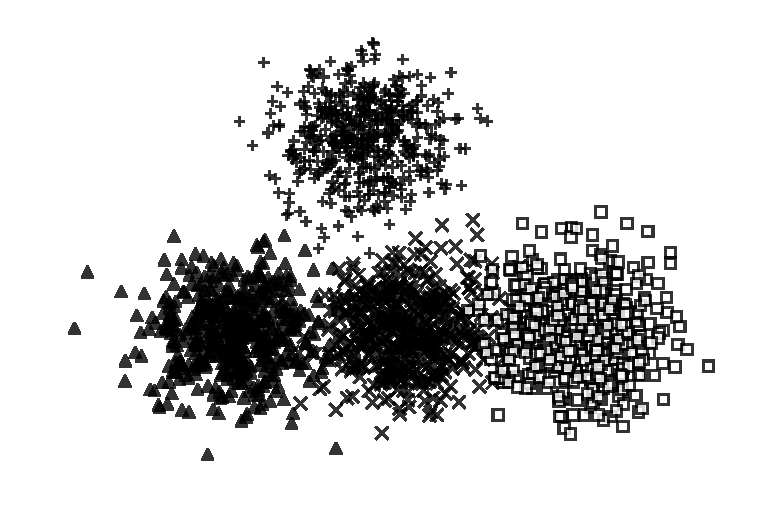
\includegraphics[width=\d cm]{dist3.pdf}};
\end{tikzpicture}

% End of code
\end{document}
